\subsection{Spectral Energy Distribution}

The \gls{sed} of galaxies is imprinted with the effects of various physical properties influencing galaxy evolution, such as metallicity, dust, grain size, \gls{sf}, and \gls{agn} activity \citep{conroy_modeling_2013}. \gls{sed} analysis has been steadily growing in popularity, which can be attributed to the influx of new data generated by extensive surveys, each encompassing thousands to millions of galaxies. Numerous SED fitting codes have been developed in the literature, including \texttt{MAGPHYS} \citep{da_cunha_simple_2008}, \texttt{EAZY} \citep{brammer_eazy_2008}, \texttt{ProSpect} \citep{leja_deriving_2017, robotham_prospect_2020}, and \texttt{CIGALE} \citep{boquien_cigale_2019}, among others. Over the past two decades, new SED codes have been made available and old ones significantly upgraded, yielding valuable insights into the evolution and formation of galaxies since the earliest epochs of cosmic history \citep{walcher_fitting_2011, conroy_modeling_2013}. 

The simultaneous interaction between the aforementioned physical factors influencing galaxy evolution combines to form the total integrated spectrum, usually spanning from the \gls{uv} to \gls{fir} wavelengths. Dust extinction absorbs outgoing \gls{uv} radiation and re-emits in the \gls{ir} regime \citep{fu_decomposing_2010, wu_mid-infrared_2011, assef_mid-ir-_2011, han_evolution_2012}. Known as energy balance \citep{smith_panchromatic_2018}, the relative incoming spectral radiance can be used to differentiate the total observed spectrum into their individual components. However, as noted by \cite{boquien_cigale_2019}, the task of modelling the observed total SED through the summation of smaller components is extremely difficult because two identical SEDs can arise from vastly different physical processes. Stellar population synthesis models are used to derive individual components to solve the degeneracy in energy balance \citep{coelho_use_2020}. This forms the basis of \gls{sed} decomposition and allows us to interpret the combination of physical factors from integrated spectra or photometry. \gls{sed} analysis is usually combined with photometry because it is already a gruelling process. While spectroscopy provides high accuracy, it is relatively slow, whereas photometry is faster, albeit less precise

\begin{figure}
    \centering
    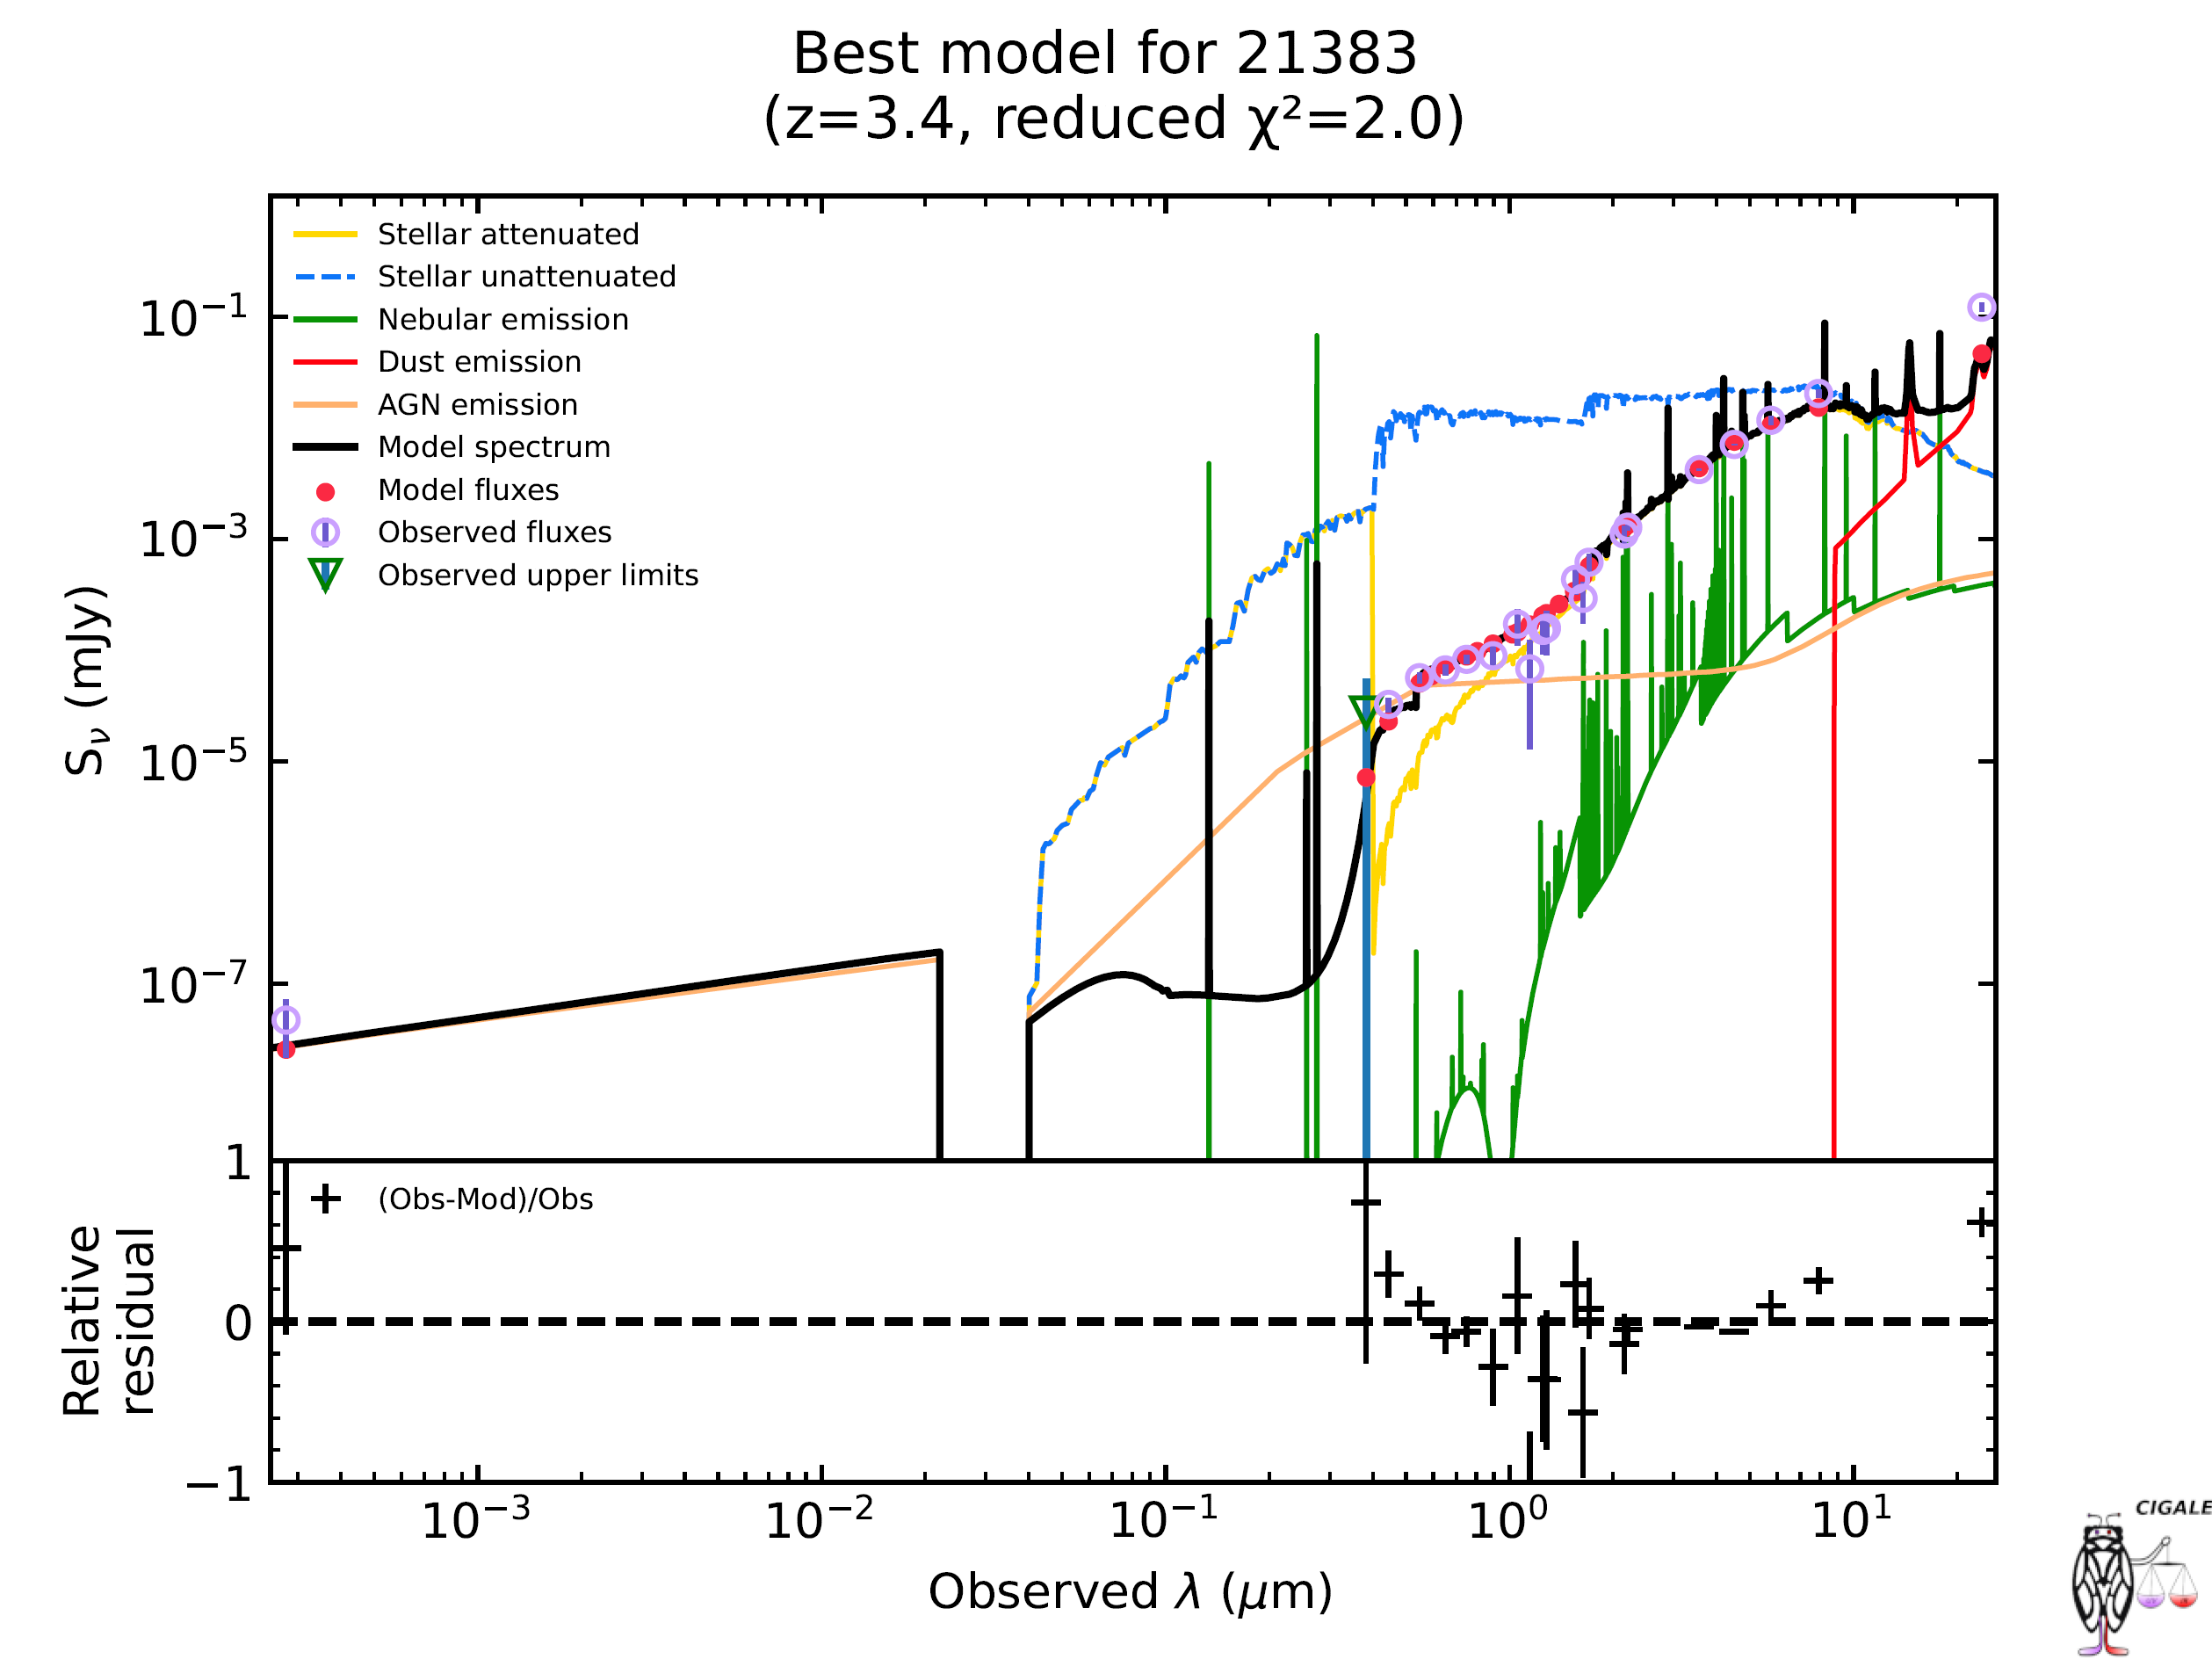
\includegraphics[width=\linewidth]{Figures/SED_Example.png}
    \caption{Example SED decomposed with CIGALE}
    \label{fig: SED}
\end{figure}

\Cref{fig: SED} presents an example galaxy spectrum from the \gls{zfourge} survey \citep{straatman_fourstar_2016} which has been decomposed into individual components using \texttt{CIGALE} \citep{boquien_cigale_2019}. The \gls{zfourge} survey aimed to observe obscured galaxies at redshifts $z>1$. This focus minimises the need for \gls{uv} wavelengths ($\lambda < \approx 1 \ \mu m$) because, as previously noted, UV light is reprocessed into the infrared (IR) range by obscuring dust. Consequently, the bolometric IR range remains, which spans from $1 < \lambda < 1000 \ \mu m$. The shape of the observed spectral energy distribution (SED) shifts with redshift, moving to shorter wavelengths as redshift increases due to the expansion of the universe. A challenge arises at high redshifts, as there have historically been few model libraries that incorporate empirical observations. Consequently, studies of high-redshift SEDs have often depended on low-redshift models to interpret their results \citep{conroy_modeling_2013, steinhardt_templates_2023}. A significant limitation of \gls{sed} modelling is whether the derived results accurately represent the true physical effects. As noted by \cite{hayward_should_2015}, independent results are often lacking to verify if an SED fitting code has accurately deduced the physical properties of a galaxy. However, conducting such verification for every galaxy would be extremely time-consuming and costly. Fortunately, a more efficient and cost-effective approach is synthetic SED validation. This process involves generating mock galaxy SEDs from simulations, which can then be tested using SED modelling codes \citep{walcher_fitting_2011, conroy_modeling_2013, hayward_should_2015, coelho_use_2020}.

Ignoring the time and cost limitations, incorporating SED decomposition is crucial for uncovering and understanding the many different evolutionary pathways galaxies take. SF and AGN activity directly probes galaxy evolution \citep{huang_local_2007, ho_spectral_1999, silva_modelling_2011, gruppioni_modelling_2011}. Decomposing the SED and recovering the AGN component, therefore, traces AGN co-evolution with the host galaxy. AGN activity is correlated with IR luminosity \citep{wu_mid-infrared_2011, symeonidis_what_2019, kauffmann_host_2003, symeonidis_agn_2021}, which introduces a bias against low-luminosity AGN and may help explain why AGN feedback is more prevalent at lower redshifts \citep{katsianis_evolution_2017, pouliasis_obscured_2020}.

Recent developments in SED software have opened new opportunities for uncovering fresh insights into galaxy evolution and AGN coevolution. \texttt{CIGALE} \citep{boquien_cigale_2019} is one of the most advanced \gls{sed} codes available, able to fit almost the entire electromagnetic spectrum, from X-ray \citep{yang_x-cigale_2020} to radio \citep{yang_fitting_2022}. New and improved perspectives on the co-evolution of galaxies and BHs will be attained using CIGALE's decomposition capabilities. 

In the existing literature, relatively few authors use \gls{sed} analysis software to decompose the AGN contribution to \gls{lf} \citep{stanley_remarkably_2015, hernan-caballero_resolving_2015, fu_decomposing_2010, gruppioni_modelling_2011, brown_infrared_2019, valiante_backward_2009}. This is due to the challenges with spectral decomposition. As \cite{silva_modelling_2011} discussed, decomposition's computational complexity is time-consuming for large data sets. Among the authors who have utilised decomposition, both \cite{fu_decomposing_2010} and \cite{brown_infrared_2019} observed that the co-evolution of \gls{agn} and \gls{sf} occurs simultaneously. Conversely, \cite{stanley_remarkably_2015} and \cite{cowley_decoupled_2018} find no correlation between AGN luminosity and SFR. However, no standardised decomposition strategy exacerbates the differences between authors and their findings \citep{wu_mid-infrared_2011}. 

In this thesis, we make use of the \texttt{CIGALE} \citep{boquien_cigale_2019} \gls{sed} fitting code to generate \gls{ir} \gls{sf} and \gls{agn} \gls{lf}s of \gls{zfourge} \citep{straatman_fourstar_2016} galaxies to analyse the formation and co-evolution of galaxies and \gls{agn}. 

% \subsection{Star Formation History}
% Test

% The SF fraction is also found to be a function of luminosity/redshift, decreasing as luminosity or redshift increases, while the trend is more obvious in the MIR, suggesting that the MIR wavelength is more sensitive to the presence of AGNs \cite{wu_mid-infrared_2011}. The IR-bright, dust-obscured galaxy population is crucial to understanding galaxy formation and evolution. \cite{gruppioni_modelling_2011}. IR bright galaxies emit the bulk of their energy as dust-reprocessed light generated by dusty SF or accretion onto the supermassive black holes referred to hereafter as active galactic nuclei. \cite{wu_mid-infrared_2011}

% \textcolor{red}{However, as \cite{katsianis_evolution_2017} reports, IR only works for dusty massive galaxies and is limited at higher redshifts. Less obscured (Type 1) galaxies may appear dimmer in the IR because they produce less light from reprocessing other wavelengths around the dusty torus.}

% \textcolor{red}{AGN light and star-forming (SF) light are two distinct components of the radiation emitted by galaxies. Understanding the relative contributions of these components is crucial for studying the energy sources and processes occurring within galaxies. Decomposing the spectral energy distribution (SED) into the component AGN and SF light has, until recently, rarely been performed, mostly because this was difficult to accomplish. Understanding the relative importance of AGN light and star-forming light is essential for characterizing the energy sources, gas dynamics, and overall evolutionary processes occurring within galaxies. It helps in unravelling the intricate connections between supermassive black holes, galaxy evolution, and the formation of stars.}